\documentclass{article}

% latex math commands
% Vladimir Feinberg
% \vx notation for vectors from Goodfellow
% https://github.com/goodfeli/dlbook_exercises

% alphabet templates
% abcdefghijklmnopqrstuvwxyz
% ABCDEFGHIJKLMNOPQRSTUVWXYZ

% fonts, math, and layout commands
\usepackage{lmodern}
\usepackage{fullpage}
\usepackage{bbm}
\usepackage{enumerate}
\usepackage{amsmath}
\usepackage{amsthm}
\usepackage{amssymb}
\usepackage{amsfonts}
\usepackage{mathrsfs}
\usepackage{mathtools}
\usepackage[all]{xy}
\usepackage{algorithm}
\usepackage[noend]{algpseudocode}

% include graphics with \includegraphics
\usepackage{graphicx}
\usepackage{caption}

% \nicefrac{x}{y} gives a diagonal fraction bar x/y
\usepackage{nicefrac}

% \nurl{<url>}{link name} renders a blue underlined link
\usepackage[hidelinks]{hyperref}
\usepackage{xcolor}
\usepackage{url}
\newcommand{\nurl}[2]{\href{ #1 }{\color{blue}\underline{#2}}}

% brackets, norms, cardinalities
\newcommand{\pa}[1]{ \left({#1}\right) }
\newcommand{\ha}[1]{ \left[{#1}\right] }
\newcommand{\ca}[1]{ \left\{{#1}\right\} }
\newcommand{\inner}[1]{\left\langle #1 \right\rangle}
\newcommand{\innercpy}[1]{\inner{ #1, #1 }}
\newcommand{\norm}[1]{\left\lVert #1 \right\rVert}
\newcommand{\card}[1]{\left\lvert{#1}\right\rvert}
\newcommand{\abs}[1]{\card{#1}}

% math vectors
\newcommand{\va}{\textbf{a}}
\newcommand{\vb}{\textbf{b}}
\newcommand{\vc}{\textbf{c}}
\newcommand{\vd}{\textbf{d}}
\newcommand{\ve}{\textbf{e}}
\newcommand{\vf}{\textbf{f}}
\newcommand{\vg}{\textbf{g}}
\newcommand{\vh}{\textbf{h}}
\newcommand{\vi}{\textbf{i}}
\newcommand{\vj}{\textbf{j}}
\newcommand{\vk}{\textbf{k}}
\newcommand{\vl}{\textbf{l}}
\newcommand{\vm}{\textbf{m}}
\newcommand{\vn}{\textbf{n}}
\newcommand{\vo}{\textbf{o}}
\newcommand{\vp}{\textbf{p}}
\newcommand{\vq}{\textbf{q}}
\newcommand{\vr}{\textbf{r}}
\newcommand{\vs}{\textbf{s}}
\newcommand{\vt}{\textbf{t}}
\newcommand{\vu}{\textbf{u}}
\newcommand{\vv}{\textbf{v}}
\newcommand{\vw}{\textbf{w}}
\newcommand{\vx}{\textbf{x}}
\newcommand{\vy}{\textbf{y}}
\newcommand{\vz}{\textbf{z}}
\newcommand{\vzero}{\textbf{0}}
\newcommand{\vone}{\textbf{1}} 
\newcommand{\valpha}{{\boldsymbol\alpha}}
\newcommand{\vepsilon}{{\boldsymbol\epsilon}}
\newcommand{\veta}{{\boldsymbol\eta}}
\newcommand{\vsigma}{ {\boldsymbol\sigma}}
\newcommand{\vtheta}{ {\boldsymbol\theta}}
\newcommand{\vdelta}{ {\boldsymbol\delta}}
\newcommand{\vlambda}{ {\boldsymbol\lambda}}
\newcommand{\vmu}{ {\boldsymbol\mu}}
\newcommand{\vvartheta}{ {\boldsymbol\vartheta}}
\newcommand{\vbeta}{ {\boldsymbol\beta}}
\newcommand{\vphi}{ {\boldsymbol\phi}}


% math function arrows, misc binary math ops
\newcommand{\bij}{\leftrightarrow}
\newcommand{\inj}{\rightarrowtail}
\newcommand{\sur}{\twoheadedrightarrow}
\newcommand{\eqd}{\mathrel{\overset{\Delta}{=}}}

% common math sets
\newcommand{\Z}{\mathbb{Z}}
\newcommand{\R}{\mathbb{R}}
\newcommand{\C}{\mathbb{C}}
\newcommand{\N}{\mathbb{N}}
\newcommand{\Q}{\mathbb{Q}}
\newcommand{\F}{\mathbb{F}}
\newcommand{\T}{\mathbb{T}}

% limits
\def\sumn{\sum_{n=0}^\infty}
\def\limn{\lim_{n\rightarrow\infty}}
\def\prodn{\prod_{n=0}^\infty}

% mathcal
\newcommand{\mcA}{\mathcal{A}}
\newcommand{\mcB}{\mathcal{B}}
\newcommand{\mcC}{\mathcal{C}}
\newcommand{\mcD}{\mathcal{D}}
\newcommand{\mcE}{\mathcal{E}}
\newcommand{\mcF}{\mathcal{F}}
\newcommand{\mcG}{\mathcal{G}}
\newcommand{\mcH}{\mathcal{H}}
\newcommand{\mcI}{\mathcal{I}}
\newcommand{\mcJ}{\mathcal{J}}
\newcommand{\mcK}{\mathcal{K}}
\newcommand{\mcL}{\mathcal{L}}
\newcommand{\mcM}{\mathcal{M}}
\newcommand{\mcN}{\mathcal{N}}
\newcommand{\mcO}{\mathcal{O}}
\newcommand{\mcP}{\mathcal{P}}
\newcommand{\mcQ}{\mathcal{Q}}
\newcommand{\mcR}{\mathcal{R}}
\newcommand{\mcS}{\mathcal{S}}
\newcommand{\mcT}{\mathcal{T}}
\newcommand{\mcU}{\mathcal{U}}
\newcommand{\mcV}{\mathcal{V}}
\newcommand{\mcW}{\mathcal{W}}
\newcommand{\mcX}{\mathcal{X}}
\newcommand{\mcY}{\mathcal{Y}}
\newcommand{\mcZ}{\mathcal{Z}}

% measure theory
\newcommand{\indicator}{\mathbbm{1}}
\DeclareMathOperator{\Laplace}{Laplace}
\DeclareMathOperator{\Poisson}{Poisson}
\DeclareMathOperator{\Exponential}{Exponential}
\DeclareMathOperator{\Multinomial}{Multinomial}
\DeclareMathOperator{\Bernoulli}{Bernoulli}
\DeclareMathOperator{\Categorical}{Categorical}
\DeclareMathOperator{\Uniform}{Uniform}
\DeclareMathOperator{\Binomial}{Binomial}
\DeclareMathOperator{\Hypergeometric}{Hypergeometric}
\DeclareMathOperator{\GammaDist}{Gamma}
\DeclareMathOperator{\NegativeBinomial}{NegativeBinomial}
\DeclareMathOperator\mathProb{\mathbb{P}}
\renewcommand{\d}[1]{\mathop{\mathrm{d} #1 }}
\DeclarePairedDelimiterX{\infdivx}[2]{(}{)}{ #1\;\delimsize\|\;#2 }
\newcommand{\dkl}[2]{\mathop{D_\text{KL}}\infdivx{#1}{#2}}

% distributions
\makeatletter
\newcommand{\distas}[1]{\mathbin{\overset{#1}{\kern\z@\sim}}}%
\makeatother
\newcommand{\disteq}{\overset{d}{=}}
\newcommand{\distiid}{\distas{\text{iid}}}
\newcommand\independent{\protect\mathpalette{\protect\independenT}{\perp}}
\def\independenT#1#2{\mathrel{\rlap{$#1#2$}\mkern2mu{#1#2}}}
\newcommand{\convdist}{\mathbin{\overset{\text{d}}{\longrightarrow}}}
\newcommand{\convas}{\mathbin{\overset{\text{as}}{\longrightarrow}}}
\newcommand{\convpb}{\mathbin{\overset{\text{pb}}{\longrightarrow}}}

\renewcommand{\P}{\mathProb} % need to overwrite stupid paragraph symbol
\DeclareMathOperator\mathExp{\mathbb{E}}
\DeclareMathOperator*\mathExpUnder{\mathbb{E}}
\newcommand{\E}{\mathExp}

\newcommand{\sa}{{$\sigma$-algebra}}
\newcommand{\OR}{{\overline{\R}}}
\newcommand{\OX}{{\overline{X}}}
\DeclareMathOperator{\power}{{\mathcal{P}}}
\DeclareMathOperator{\var}{var}
\DeclareMathOperator{\cov}{cov}

% \set{from set}{condition} with set-builder notation
% conditional expectation is analogous
\newcommand{\set}[2]{ \left\{ #1 \,\middle|\, #2 \right\} }
\newcommand{\CE}[2]{ \mathExp\left[ #1 \,\middle|\, #2 \right] }

% linear-algebra related
\newcommand{\mat}[1]{\begin{pmatrix} #1 \end{pmatrix}}
\newcommand{\detmat}[1]{\begin{vmatrix} #1 \end{vmatrix}}
\DeclareMathOperator{\spanb}{span}
\DeclareMathOperator{\conv}{conv} % convex hull
\DeclareMathOperator{\cone}{cone}
\DeclareMathOperator{\vectorize}{vec}
\DeclareMathOperator{\matricize}{mat}
\DeclareMathOperator{\adj}{adj}
\DeclareMathOperator{\diag}{diag}
\DeclareMathOperator{\tr}{tr}
\DeclareMathOperator{\rank}{rank}
\DeclareMathOperator*{\argmin}{argmin}
\DeclareMathOperator*{\argmax}{argmax}
\DeclareMathOperator*{\proj}{proj}

% complex analysis
\DeclareMathOperator{\MyRe}{Re}
\DeclareMathOperator{\MyIm}{Im}
\DeclareMathOperator{\image}{image}
\DeclareMathOperator{\supp}{supp}

% typical numerical operators
\DeclareMathOperator{\sgn}{sgn}

% graphs
\DeclareMathOperator{\diam}{diam}

% constants
\renewcommand{\d}[1]{\mathop{\mathrm{d} #1 }}
\newcommand{\e}{\mathrm{e}}
\renewcommand{\i}{\imath}

% \bigtimes: large indexed cross product
\makeatletter
\DeclareFontFamily{U}  {MnSymbolF}{}
\DeclareSymbolFont{symbolsMN}{U}{MnSymbolF}{m}{n}
\SetSymbolFont{symbolsMN}{bold}{U}{MnSymbolF}{b}{n}
\DeclareFontShape{U}{MnSymbolF}{m}{n}{
    <-6>  MnSymbolF5
   <6-7>  MnSymbolF6
   <7-8>  MnSymbolF7
   <8-9>  MnSymbolF8
   <9-10> MnSymbolF9
  <10-12> MnSymbolF10
  <12->   MnSymbolF12}{}
\DeclareFontShape{U}{MnSymbolF}{b}{n}{
    <-6>  MnSymbolF-Bold5
   <6-7>  MnSymbolF-Bold6
   <7-8>  MnSymbolF-Bold7
   <8-9>  MnSymbolF-Bold8
   <9-10> MnSymbolF-Bold9
  <10-12> MnSymbolF-Bold10
  <12->   MnSymbolF-Bold12}{}
\DeclareMathSymbol{\tbigtimes}{\mathop}{symbolsMN}{2}
\newcommand*{\bigtimes}{%
  \DOTSB
  \tbigtimes
  \slimits@ 
}
\makeatother

% category theory arguments
% See https://tex.stackexchange.com/questions/356873
\newcommand{\catfst}{{-}}
\newcommand{\catsnd}{{=}}
\newcommand{\cattrd}{{\equiv}}
\DeclareMathOperator{\Id}{Id}
\newcommand{\opcat}[1]{{#1}^{\text{op}}}
\DeclareMathOperator{\Hom}{hom}
\DeclareMathOperator{\Ob}{ob}
\DeclareMathOperator{\El}{el}
\DeclareMathOperator{\colim}{colim}
\DeclareMathOperator{\Sym}{Sym}

% references
\newcommand{\figref}[1]{Figure~\ref{fig:#1}}
\newcommand{\tabref}[1]{Table~\ref{tab:#1}}
\newcommand{\secref}[1]{Section~\ref{sec:#1}}
\newcommand{\equref}[1]{Equation~\ref{eq:#1}}
\renewcommand{\algref}[1]{Algorithm~\ref{alg:#1}}

% centered figure with \autofig{filepath}{\label{fig:somelabel}}{caption}
\newcommand{\autofig}[3]{
  \begin{figure}[!ht]
    \begin{center}
      \includegraphics[width=0.8\columnwidth]{#1}
    \end{center}
    \caption{#3}
    #2
\end{figure}
}

\usepackage{fancyvrb}
\usepackage{verbatimbox}
\usepackage{placeins}
\title{Bootstrapped MPC\\\large CS 294-112}
\author{Vladimir Feinberg, Samvit Jain, Michael Whittaker}
\date{10 October 2017}

\begin{document}
	
\maketitle

\section{Smarter Sampling}\label{smart-sample}

We consider learning the dynamics for the \texttt{HalfCheetah-v1} environment and using those dynamics to simulate rollouts with random actions, taking the action that resulted in the lowest cost after the simulation.

Unless otherwise specified, all parameters are their defaults: 5 different seeds (TODO: for now only 1) for each setup, 60 epochs of dynamics training on the full dataset per on-policy iteration, a dynamics batch size of 512, maximum episode length of 1000, 1000 simulated paths in the MPC controller (each of which has a horizon of 15), and 10 paths sampled by the initial random agent and then by the MPC controller that are aggregated every policy iteration. The learning rate was the default $10^{-3}$.

Instead of random sampling during the simulations, one might attempt to have a more intelligent MPC rollout. In particular, we can have a policy learn the from the MPC expert: every iteration we train a neural network from our aggregated policy to mimic the MPC rollout. Then, when we sample, we use MPC control, but only with the first action randomly sampled at uniform. All then next actions are taken by the learned policy. By having more reasonable simulated rollouts, MPC can choose smarter initial actions. The neural network training wasn't a noticeable additional time cost, but resulted in much-improved performance (Fig.~\ref{fig:mpcmf}).

\begin{figure}[!h]
  \begin{center}
    {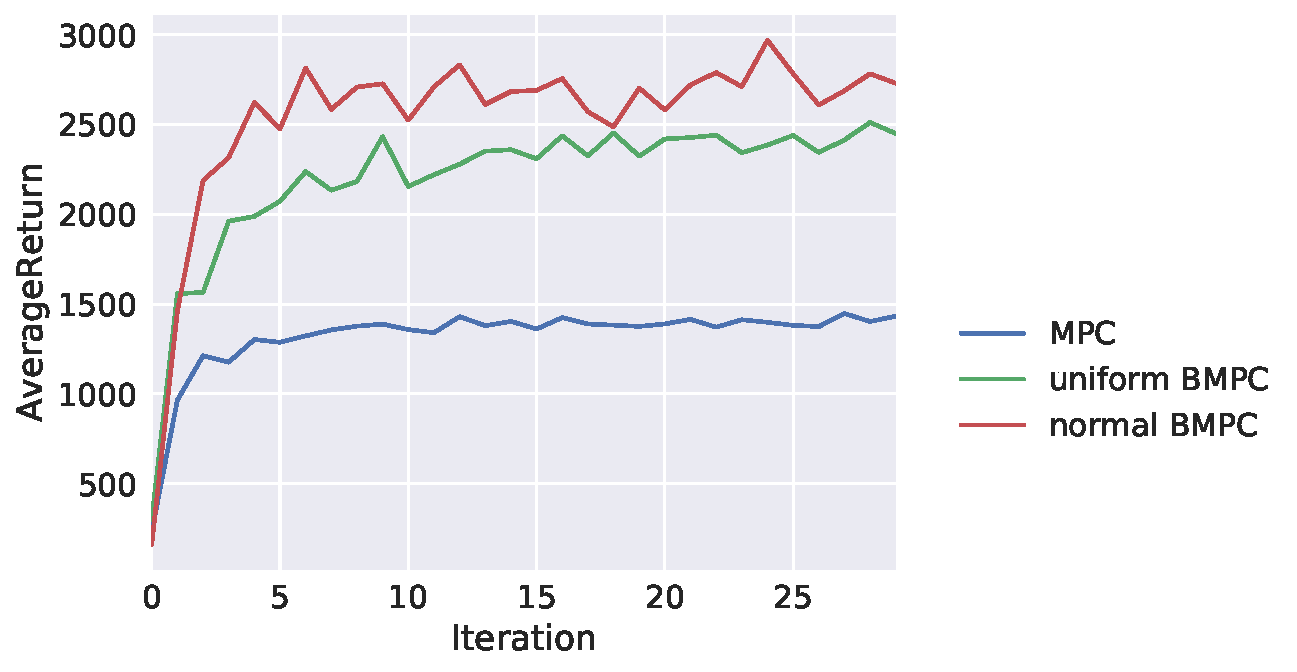
\includegraphics[width=0.8\textwidth]{easy-AverageReturn.pdf}}
  \end{center}
  \caption{Average return over policy aggregation iterations for the learning-based sampling MPC agent, compared to the standard uniform sampling MPC agent.}
\label{fig:mpcmf}
\end{figure}

This results in a pretty interesting ``bootstrapping'' effect where the MPC expert gets better by relying on what is essentially a memoized version of itself. Note that the learner neural network is only used starting on the second step of the MPC rollout simulations, with the first one still randomly sampled. This strategy seems pretty similar to MCTS, but in a continuous setting (where we have a policy picking the action to take).

In Figure~\ref{fig:mpcmf}, we consider the first action to not just be random, but also random and sampled normally around the learned policy. Figure~\ref{fig:mpcmf} uses a policy provided in the homework. If we don't use the homework's policy, which encodes supervision in the cost function (bad cheetah posture was penalized explicitly), we can only rely on the usual \texttt{HalfCheetah-v1} reward. This makes problem significantly harder.

In this case, bootstrapping still helps (Figure~\ref{fig:hardcost}).

\begin{figure}[!h]
  \begin{center}
    {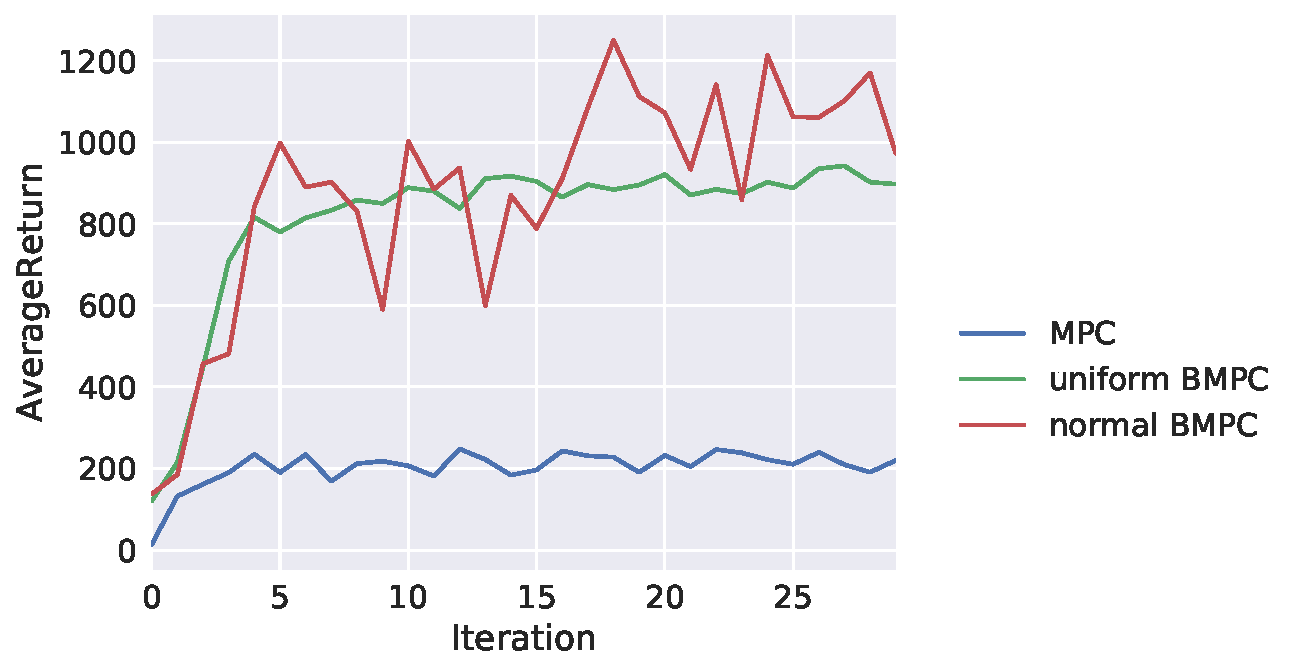
\includegraphics[width=0.8\textwidth]{hard-AverageReturn.pdf}}
  \end{center}
  \caption{Average return over policy aggregation iterations for the learning-based sampling MPC agent, compared to the standard uniform sampling MPC agent, this time with a hard cost function.}
\label{fig:hardcost}
\end{figure}


\FloatBarrier

\section{Conclusion}

I expect that it may be possible to speed up test-time execution by using the learned policy network mentioned in Sec.~\ref{smart-sample}, with a DAGGER-style approach as mentioned in the paper: use the learned policy network to make sampling decisions, and only rely on the MPC controller (perhaps using the policy network for sampling again) for expert annotations. When I tried this, I found that the policy network did not have variable-enough performance to explore sufficiently. Perhaps this was just a matter of messing with variance hyperparameters for the learned network's Gaussian policy, but I tried quite a few. I noticed that the paper mentioned in the assignment warm-started the dataset with (randomly-sampled) MPC samples (whereas I did a cold-start from training on expert-labelled states generated by the random agent). Perhaps the warm-start was key, but it feels like cheating, since you need to run your MPC samples anyway.

\end{document}
